\chapter{Problema e Proposta}


\section{Problema}
	O problema que nos propomos a resolver se refere ao fato do \textit{middleware} chamado \textit{UbiquitOS} não ter capacidade de reconhecer, de forma não intrusiva, a presença, identificação e localização de usuários dentro do \textit{SmartSpace}.

	Essas informações são importantes para o \textit{middleware}, pois para conseguir uma boa interação entre as diversas peças que compõem o \textit{SmartSpace} é necessário que se tenha a disposição informações de contexto. Informações de contexto são importantes para definir ajustes finos nos componentes do ambiente, como, por exemplo, definir o identificar perfis do usuário e, a partir do mesmo, ajustar os dispositivos presentes no ambiente.

\section{Proposta}

	Nosso objetivo é propor um sistema eficiente para reconhecimento e localização de usuários dentro de um \textit{SmartSpace} em tempo real. Para alcançar esse objetivo iremos implementar um sistema eficiente que, através de imagens de cor e de profundidade providas pelo \textit{Kinect} e utilizando as bibliotecas \textit{OpenCV} e \textit{OpenNI}, reconheça e rastreie os usuários durante a sua permanência no \textit{SmartSpace}.


	Ao todo usaremos 4 \textit{Kinects} dispostos conforme a Figura \ref{smartSpaceProposto}. Essa disposição foi definida para evitar problemas de obstrução de usuários que podem atrapalhar o reconhecimento e o rastreamento dos usuários e também para maximizar o alcance dos \textit{Kinects} e aumentar a robustez graças a redundância de dados.

	\begin{figure}[hbt]
		\begin{center}
			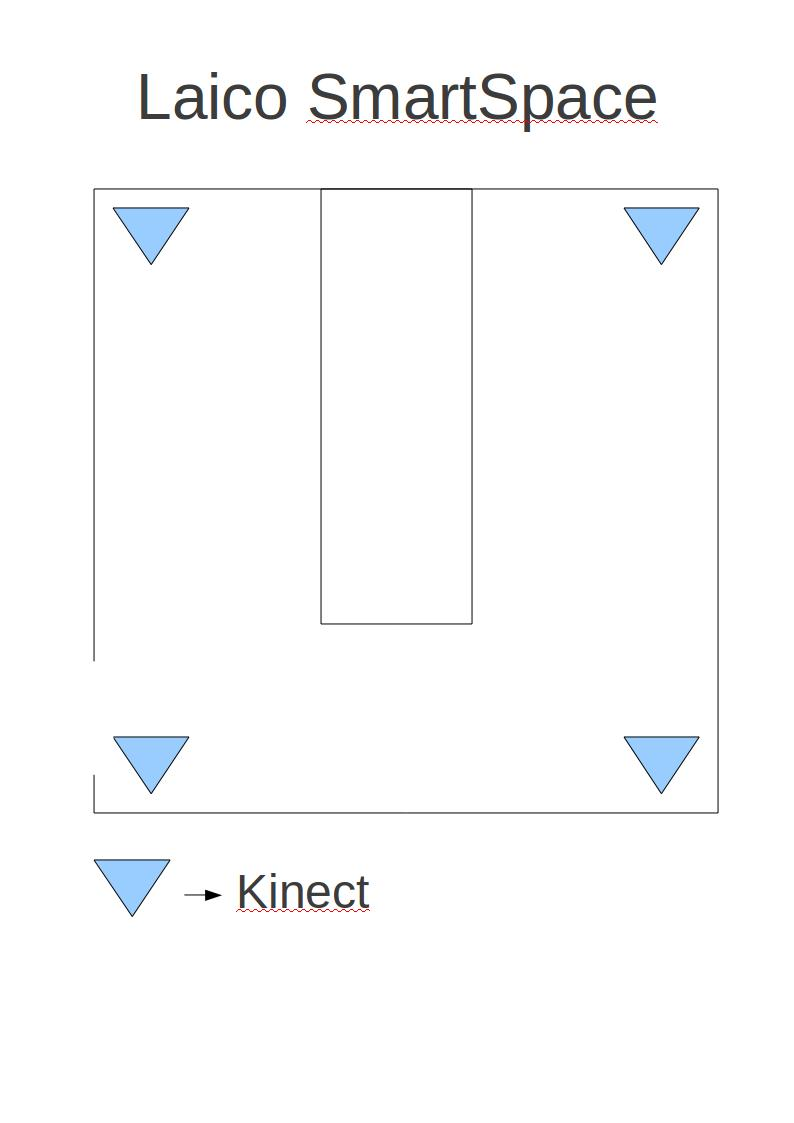
\includegraphics[scale=0.3]{figuras/4.ProblemaEProposta/esquemaSmartSpaceProposto.jpg}
		\end{center}
		\caption{Esquema proposto para o \textit{SmartSpace} com \textit{Kinect}.}
		\label{smartSpaceProposto}
	\end{figure}

	Para detecção de faces utilizaremos o método de \textit{Viola-Jones} e para o reconhecimento facial utilizaremos \textit{Eigenfaces}. Ambos os métodos já são implementados pela biblioteca \textit{OpenCV} (\textit{Open Source Computer Vision}), que é uma biblioteca aberta para computação visual muito utilizada. Estes métodos serão aplicados nas imagens de cor providas pela câmera de cor do \textit{Kinect}.

	Para localização e rastreamento dos usuários no \textit{SmartSpace} utilizaremos a biblioteca \textit{OpenNI} (\textit{Open Natural Interaction}). Esta é uma biblioteca aberta que define APIs para o desenvolvimento de aplicações utilizando interação natural. A API padrão permite aos desenvolvedores rastrear cenas (3D) da vida real, utilizando tipos de dados que são calculados a partir da entrada de um sensor, como por exemplo: a representação de um corpo completo, a representação da localização da mão, uma matriz de  \textit{pixels} em mapa de profundidade e assim por diante~\cite{openni}. Com isso, utilizaremos essa API e as imagens de profundidade providas pelas câmeras de profundidade do \textit{Kinect}, para rastrear e localizar os usuários em tempo real.

	A partir dessa proposta esperamos que o nosso sistema funcione em tempo real e que tenha o índice mínimo de confiança de 95\%. 